\chapter{Analysis and Reconstruction of Dileptonic Top-Quark Pair Events}
\label{chap:reconstruction-methods}
\section{Data and Simulation}
\label{sec:data-and-simulation}

This section describes the data and simulation samples used in this analysis. At the current stage of this thesis, only simulation samples have been studied; the data samples will be described in the final version. The simulated samples are produced using Monte Carlo (MC) event generators as described in \Cref{sec:mc_training_data}.

While a complete analysis requires detailed investigation of background processes contributing to the signal regions, this thesis focuses on developing and evaluating reconstruction methods. Therefore, only the signal process of \ttbar production with dileptonic decays is described here. The background processes and their simulation will be discussed in the final thesis.

\subsection{Simulation of Dileptonic Top-Quark Pair Events}
\label{sec:nominal_ttbar}
The signal process of \ttbar production with dileptonic decays is simulated using \powheg~\cite{powheg} at next-to-leading order (NLO) in perturbative quantum chromodynamics (QCD). The \powheg generator is interfaced with \pythia~\cite{pythia} for parton showering, hadronization, and underlying event modelling.

To link the reco-level particles to the parton-level objects, a parton matching is performed. The parton-level objects are defined as the top quarks and their decay products after final state radiation before hadronization. The matching is done by iteratively associating reconstructed jets to partons based on angular distance criteria. The decay products of the top quarks are matched within a cone of $\Delta R \leq 0.3$ and $\Delta R\leq 0.1$ for jets and leptons ($e$,$\mu$) respectively. If multiple reconstructed objects are found within this cone, the one with the smallest $\Delta R$ is chosen.

\subsection{Simulation of Non-Relativistic Quasi-Bound State Resonance}



\subsection{Object Definition}
\label{sec:object-definition}
The reconstruction of physics objects—electrons, muons, jets, and missing transverse energy (\met)—is performed using the standard \atlas reconstruction algorithms~\cite{atlas_tdr}.

\paragraph{Electrons} are required to have transverse momentum \pt $> 5~\unit{\giga\electronvolt}$ and pseudorapidity $|\eta| < 2.47$, excluding the transition region between the barrel and endcap calorimeters ($1.37 < |\eta| < 1.52$). Electrons must satisfy the Tight identification criteria and be isolated from other activity in the detector.

\paragraph{Muons} are reconstructed using information from both the inner detector and the muon spectrometer. They are required to have \pt $> 5~\unit{\giga\electronvolt}$ and $|\eta| < 2.5$. Muons must satisfy the Tight identification criteria and be isolated.

\paragraph{Jets} are reconstructed using the anti-$k_t$ algorithm \cite{anti_k_t_jet_2} with a radius parameter of $R = 0.4$. They are required to have \pt $> 25~\unit{\giga\electronvolt}$ and $|\eta| < 2.5$. $b$-tagging is performed using the GN2 algorithm~\cite{gn2_btagger} to identify jets originating from $b$-quarks.

\paragraph{Missing Transverse Energy} (\met) is calculated from the negative vector sum of the transverse momenta of all reconstructed objects in the event, including a soft term to account for energy not associated with reconstructed objects.

\subsection{Event Selection}
\label{sec:event-selection}
Events are selected to contain exactly two oppositely charged leptons (electrons or muons). One of the leptons must have \pt $> 25~\unit{\giga\electronvolt}$, while the other must have \pt $> 5~\unit{\giga\electronvolt}$. At least two jets are required, with at least one being $b$-tagged at the $77\%$ working point (WP). Additional selection criteria are applied to suppress background contributions, which will be detailed in the final thesis.

For the training and evaluation of the reconstruction methods, only events that pass the selection criteria and have a successful parton matching are considered. Fully parton-matched events, make up about $60\%$ of the whole sample. Events with jets or leptons of the \ttbar-process end up outside the detector acceptance are typically the main cause for an event being unmatchable. Thus, training with only parton-matched events might introduce a bias with respect to certain event topologies, if they are disfavoured to have a parton-matching.


\section{Reconstruction of Top-Quark Pairs}
\label{sec:reconstruction-methods}
Reconstructing the kinematics of dileptonic \ttbar events requires an assignment of reconstructed objects to the parton-level decay products. This section describes the different reconstruction methods developed and evaluated in this thesis.

While the leptons are directly identified from the reconstructed objects, the assignment of jets to the $b$-quarks from the top quark decays is ambiguous due to the presence of multiple jets in the event. Additionally, the two neutrinos from the $W$ boson decays are not directly detected, leading to missing information in the event reconstruction.
Based on this, the reconstruction breaks down into two main tasks:
\paragraph{Jet Assignment} Assigning the reconstructed jets to the $b$-quarks from the top quark decays.
\paragraph{Neutrino Regression} Estimating the momenta of the two neutrinos using the measured \met and other event kinematics.

\subsection{B-Tagging}
\label{sec:b_tagging}
The identification of $b$-jets is crucial for the reconstruction of \ttbar events. Due to the long lifetime of $b$-hadrons, they travel a measurable distance from the primary vertex before decaying, leading to displaced vertices and tracks with large impact parameters. The GN2 algorithm \cite{gn2_btagger} is used for $b$-tagging in this analysis, which combines various discriminating variables using a deep (graph) neural network to achieve high efficiency and purity in identifying $b$-jets. The performance of the $b$-tagging algorithm is characterised by its efficiency (the probability of correctly identifying a $b$-jet) and its misidentification rate (the probability of incorrectly tagging a non-$b$-jet as a $b$-jet).


\subsection{Jet Assignment Methods}
\label{sec:jet_assignment}
This thesis explores several methods for jet assignment, ranging from traditional algorithms to machine learning approaches. While the leptons can be assigned to the $W$ bosons based on their charge, the assignment of jets to the $b$-quarks is not straightforward due to the presence of multiple jets in the event. All the methods presented here, utilise kinematic relationships to make an assignment which jet and lepton stem from the same top quark decay.
From recent publications e.g. \cite{ATLAS2024Entanglement}, two conventional methods have been implemented as baselines:

\paragraph{Jet-Selection}
Both methods start by selecting the two $b$-jet candidates in the event based on the $b$-tagging at the $77\%$ WP. If more than two $b$-tagged jets are present, the two with the highest \pt are chosen. If only one $b$-tagged jet is found, the non-tagged jet with the highest $b$-tagging score is selected as the second candidate.
\begin{figure}[H]
    \centering
    \begin{minipage}[t]{0.48\textwidth}
        \textbf{$\chi^2$-Method}\\[0.5em]
        For both possible assignments of the two $b$-jet candidates to the parton-level $b$-quarks, the invariant masses of the reconstructed top quarks are computed,
        \begin{equation}
            \label{eq:chi_square}
            \chi^2 = (m_{b_1,{\nu},\ell^+} - m_{t})^2+(m_{b_2,\bar{\nu},\ell^-} - m_{t})^2
        \end{equation}
        where $m_t = 172.5~\unit{\giga\electronvolt}$ is the top quark mass. The assignment with the smaller $\chi^2$ value is chosen.
    \end{minipage}
    \hfill
    \begin{minipage}[t]{0.48\textwidth}
        \textbf{$\Delta R$-Method}\\[0.5em]
        This method assigns the $b$-jet candidates based on their angular distance to the leptons.
        \begin{equation}
            \Delta R = \sqrt{(\Delta\phi)^2 + (\Delta\eta)^2}
        \end{equation}
        The jet-lepton-pair with the smaller $\Delta R$ value is assigned to each other. The remaining jet is assigned to the other lepton.
    \end{minipage}
\end{figure}
Note, that the $\chi^2$-Method relies on the reconstructed neutrino momenta to compute the invariant masses of the top quarks. Therefore, it is inherently linked to the neutrino regression method used. In contrast, the $\Delta R$-Method is independent of the neutrino momenta.
For the analysis here, the regression from $\nu^2$-Flows was found to deliver a much better performance for the assignment. Thus, ultimately, the $\chi^2$-Method was used in conjunction with the prediction of $\nu^2$-Flows instead of the $\nu$-Weighter to provide a reasonable baseline.

Empiric evidence for the validity of both can be found in \Cref{fig:jet_lepton_pairing}, which shows the distributions of the reconstructed invariant mass of the top quark and the $\Delta R$ between the jet and lepton for correct and incorrect jet-lepton pairs. The correct pairs show a clear peak around the top quark mass in the invariant mass distribution and a smaller $\Delta R$ compared to incorrect pairs, which supports the use of these variables for jet assignment.

The $\Delta R$-Method was used in previous \atlas analyses \cite{ATLAS2024Entanglement} for events, that failed the kinematic reconstruction required for the $\chi^2$-Method. However, in this thesis, both methods are evaluated on the full dataset for comparison. 

\begin{figure}
    \centering
    \begin{subfigure}{0.49\textwidth}
        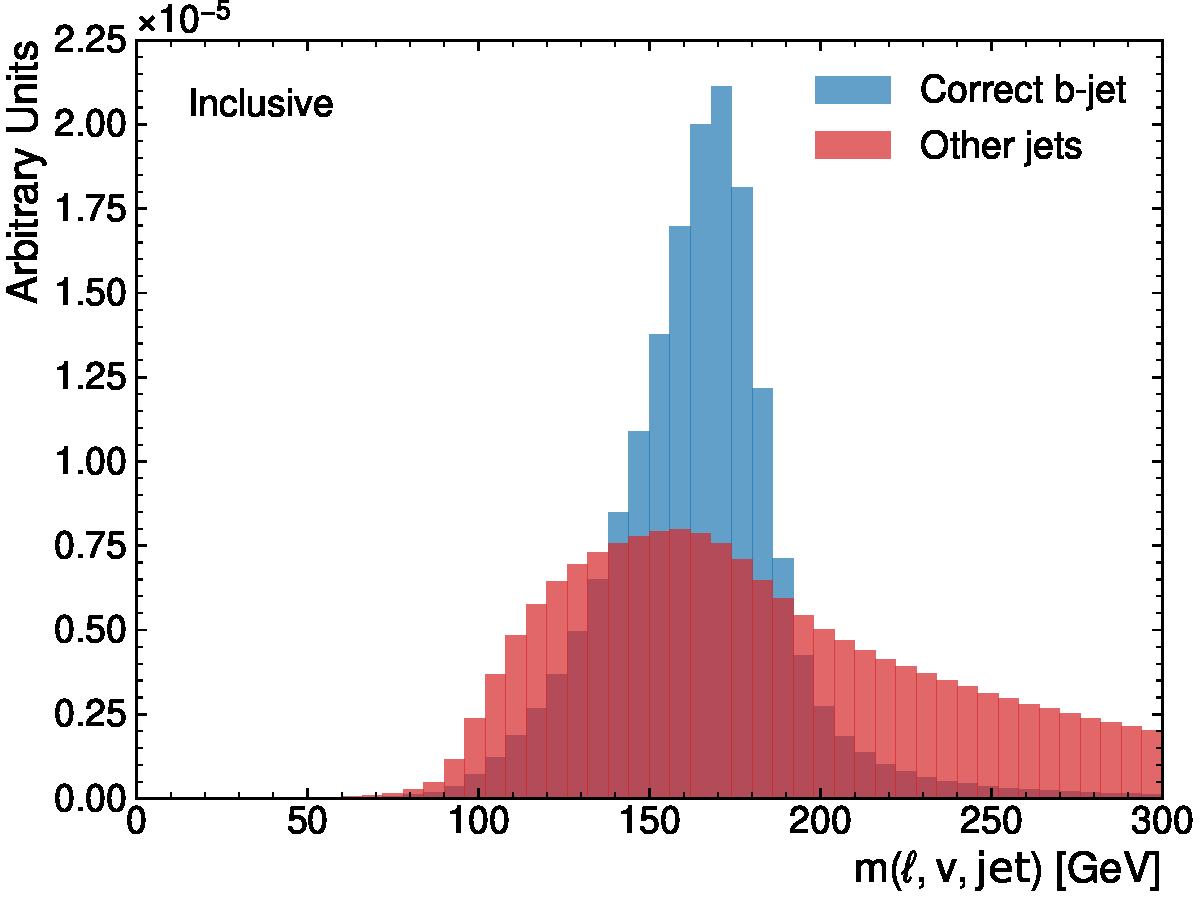
\includegraphics[width=\textwidth]{plots/feature_plots/relational_jet_lepton_full_inv_mass_distribution.pdf}
        \caption{$\chi^2$-Method}
        \label{subfig:chi_square_method}
    \end{subfigure}
    \begin{subfigure}{0.49\textwidth}
        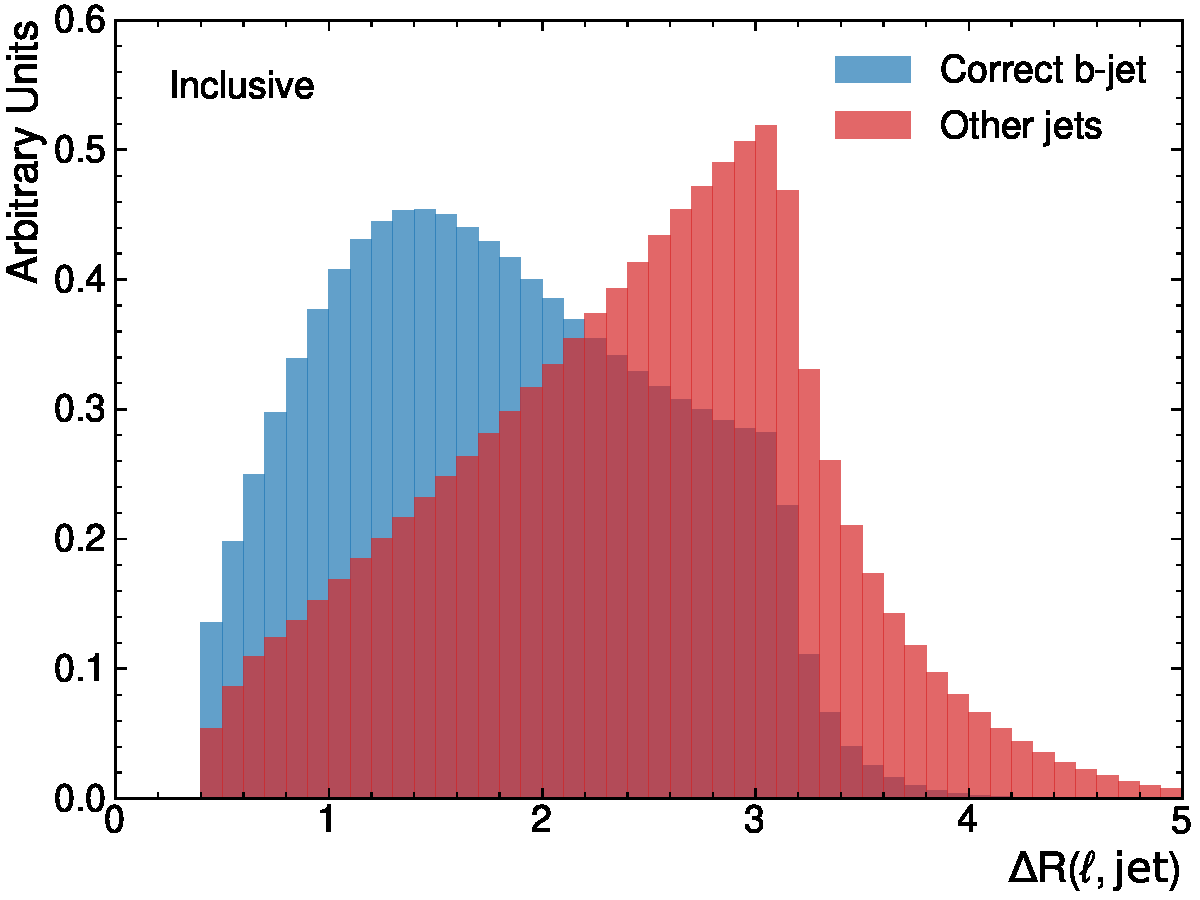
\includegraphics[width=\textwidth]{plots/feature_plots/relational_jet_lepton_deltaR_distribution.pdf}
        \caption{$\Delta R$-Method}
        \label{subfig:delta_R_method}
    \end{subfigure}
    \caption{Distributions for pairing up correct and incorrect jet-lepton pairs for the reconstructed invariant mass of the top quark (a) and the $\Delta R$ between the jet and lepton (b). The correct pairs are shown in blue, while the incorrect pairs are shown in red. The distributions are normalised to unit area. Note, that the reconstructed invariant mass for the $\chi^2$-Method includes the neutrino prediction from $\nu^2$-Flows.}
    \label{fig:jet_lepton_pairing}
\end{figure}

\subsection{Neutrino Regression Methods}
\label{sec:neutrino_regression}
Due to the limited availability of kinematic reconstruction methods in the \atlas software framework, two methods for neutrino regression are implemented and evaluated in this thesis. For completeness, the Ellipse-method, which has been used in previous \atlas analyses is described as well, but they have not been implemented or evaluated in this thesis.


\subsubsection{Ellipse-Method}
The ellipse method \cite{ellipse_method} is a kinematic reconstruction technique that exploits the constraints of the event to solve for the neutrino momenta. The method uses the measured \met and the momenta of the leptons and jets to construct a system of equations based on the invariant mass constraints of the $W$ bosons and top quarks. By solving this system of equations, one can obtain possible solutions for the neutrino momenta. The method typically yields multiple solutions, and additional criteria are used to select the most likely solution based on the event kinematics. In previous \atlas analyses, the solution yielding the lowest $m(t\bar{t})$ was chosen as the reconstructed neutrino momenta.

\subsubsection{Neutrino-Weighter}
The Neutrino-Weighter ($\nu$-Weighter), first described in \cite{neutrino_weighting_method}, is a method that assigns weights to different possible neutrino momentum configurations based on how well they satisfy the kinematic constraints of the event. The method uses the measured \met and the momenta of the leptons and jets to compute a weight for each possible neutrino momentum configuration. For each configuration, a weight is computed based on how well the reconstructed event kinematics match the expected kinematics of a \ttbar event - this includes constraints such as the invariant mass of the $W$ bosons and top quarks. The configuration with the highest weight is then selected as the reconstructed neutrino momenta. This method is computationally intensive, as it requires scanning over numerous possible neutrino momentum configurations. The computation of the reconstructed masses for the tops and W-bosons requires identification of the jets with a lepton. In principle this might be done by a sophisticated method such as the ones presented here.
However, the implementation used here, selected the jets based on b-tagging at $85\%$ working-point, and leading $p_T$ in case, the number of b-tagged jets deviates from two. While this still leaves a two-fold degeneracy for the assignment, both of the scenarios were evaluated, weighted and considered for the maximisation of the likelihood.

\subsubsection{$\nu^2$-Flows}
The method $\nu^2$-Flows \cite{nu_square_flows} uses normalizing flows to model the conditional probability distribution of the neutrino momenta given the observed event kinematics. The model is trained on simulated dileptonic \ttbar events, where the true neutrino momenta are known from the parton-level information. The trained model can then be used to sample possible neutrino momenta for new events, allowing for a probabilistic reconstruction of the event kinematics. For each event, multiple samples of neutrino momenta are drawn from the model, and the one with the highest probability density is selected as the reconstructed neutrino momenta.
A detailed outline of the $\nu^2$-Flows method and its implementation can be found in Reference~\cite{nu_square_flows}. For this thesis, this method serves to establish a baseline for neutrino regression to evaluate the impact of improved jet assignment methods. Note, however, that this method has not been used in \atlas analyses yet. However, due to matters of software compatibility, it was one of the only viable options at this stage of the thesis.
Since $\nu^2$-Flows processes the full event information to make a prediction for the neutrino momenta, it does not require a jet-assignment. Therefore, it can be used in conjunction with both the $\chi^2$-Method and the $\Delta R$-Method for jet assignment, allowing for a direct comparison of the impact of the jet assignment on the overall reconstruction performance.